\section{Appendix}

\subsection{Appendix A - Previous design work}
\label{sec:AppendixA}

  \begin{figure}[H]
    \centering
    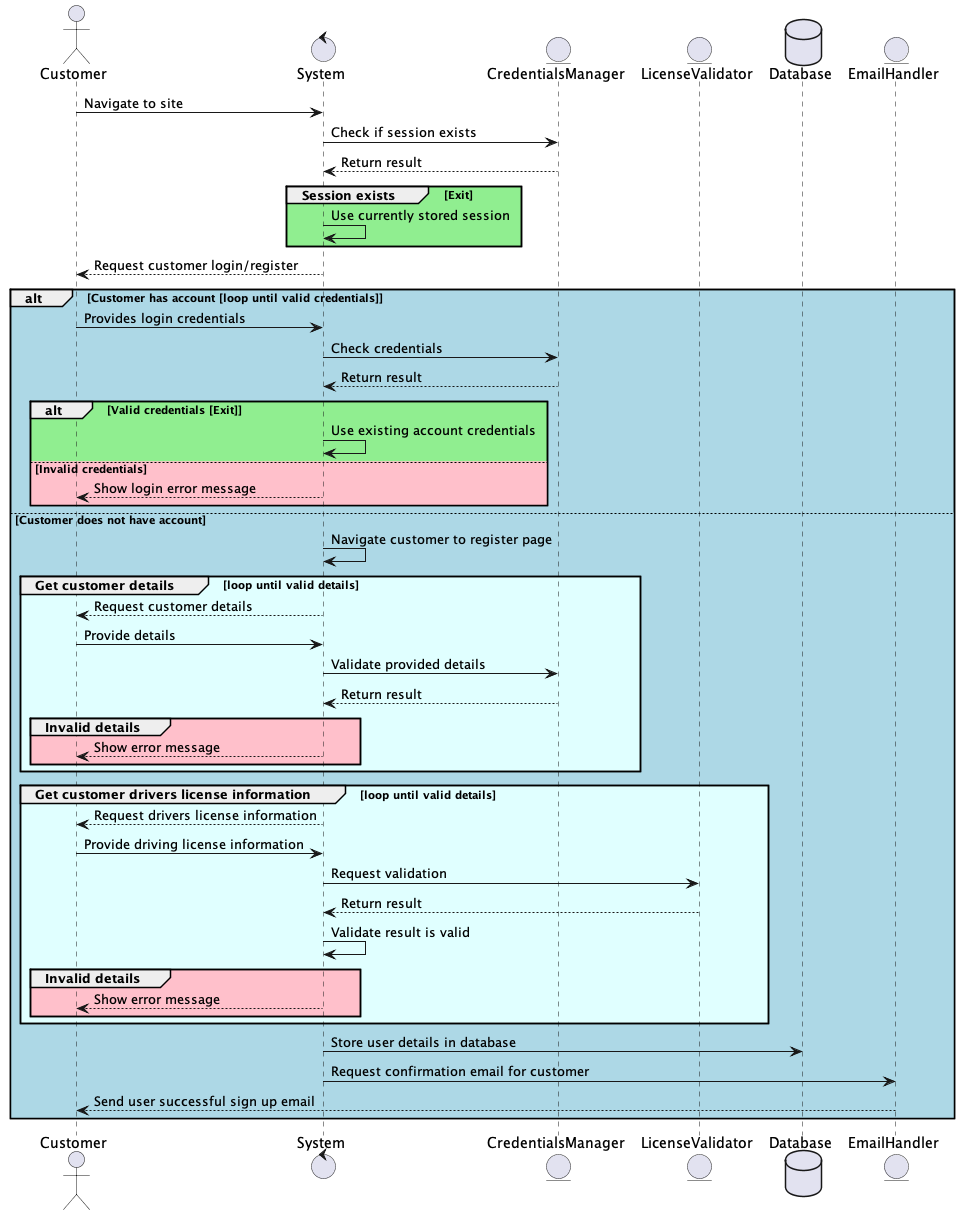
\includegraphics[width=12cm]{assets/Sequence1.png}
    \caption{Sequence diagram for adding a new user, this includes sign in/up.}
    \label{fig:newUserSequence}
  \end{figure}

  \begin{figure}[H]
    \centering
    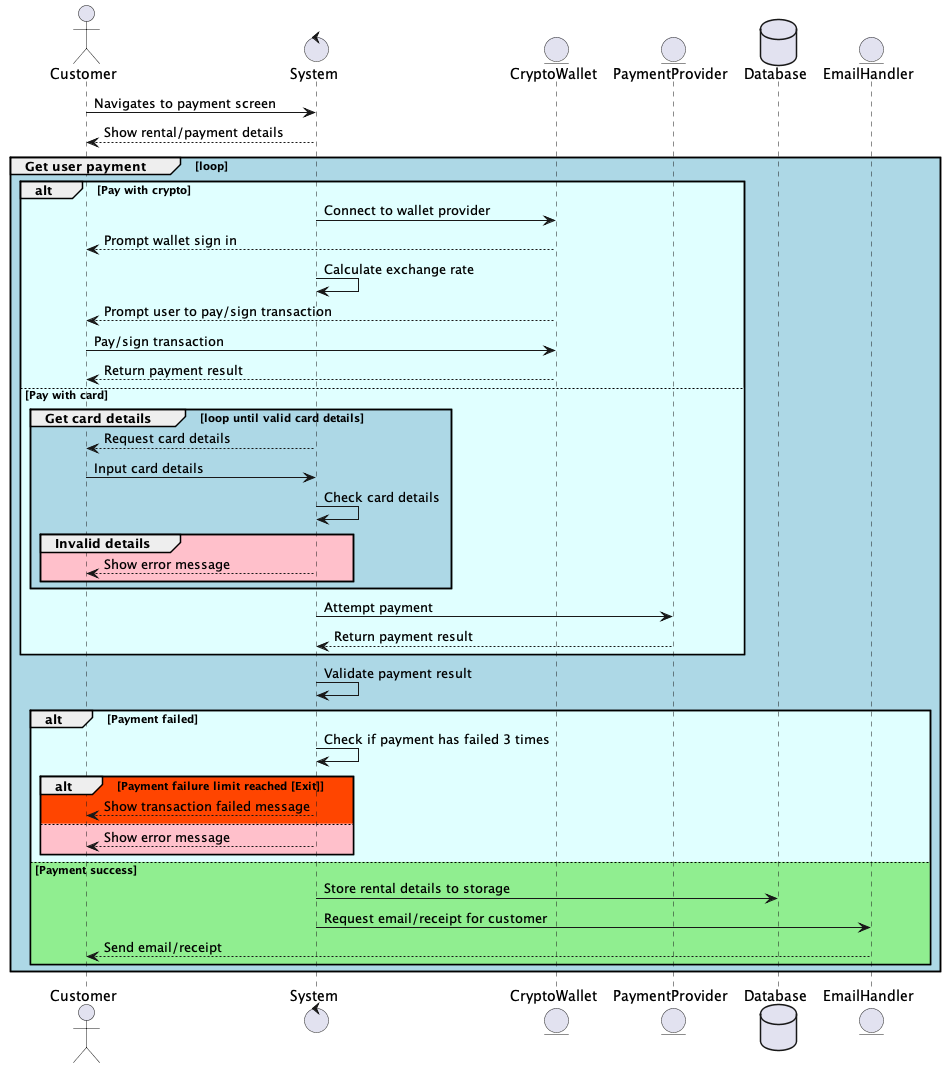
\includegraphics[width=12cm]{assets/Sequence2.png}
    \caption{Sequence diagram for taking a payment.}
    \label{fig:takePaymentSequence}
  \end{figure}

  \begin{figure}[H]
    \centering
    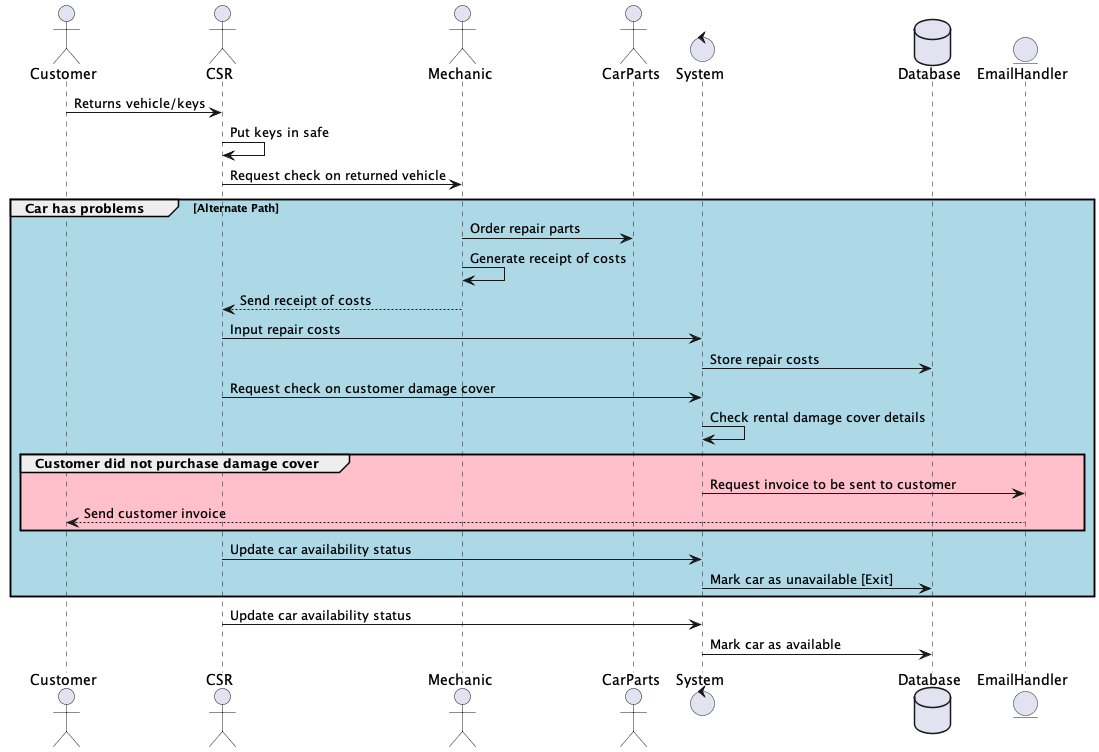
\includegraphics[width=12cm]{assets/Sequence3.png}
    \caption{Sequence diagram for handling the return of a vehicle.}
    \label{fig:vehicleReturnSequence}
  \end{figure}

  \begin{figure}[H]
    \centering
    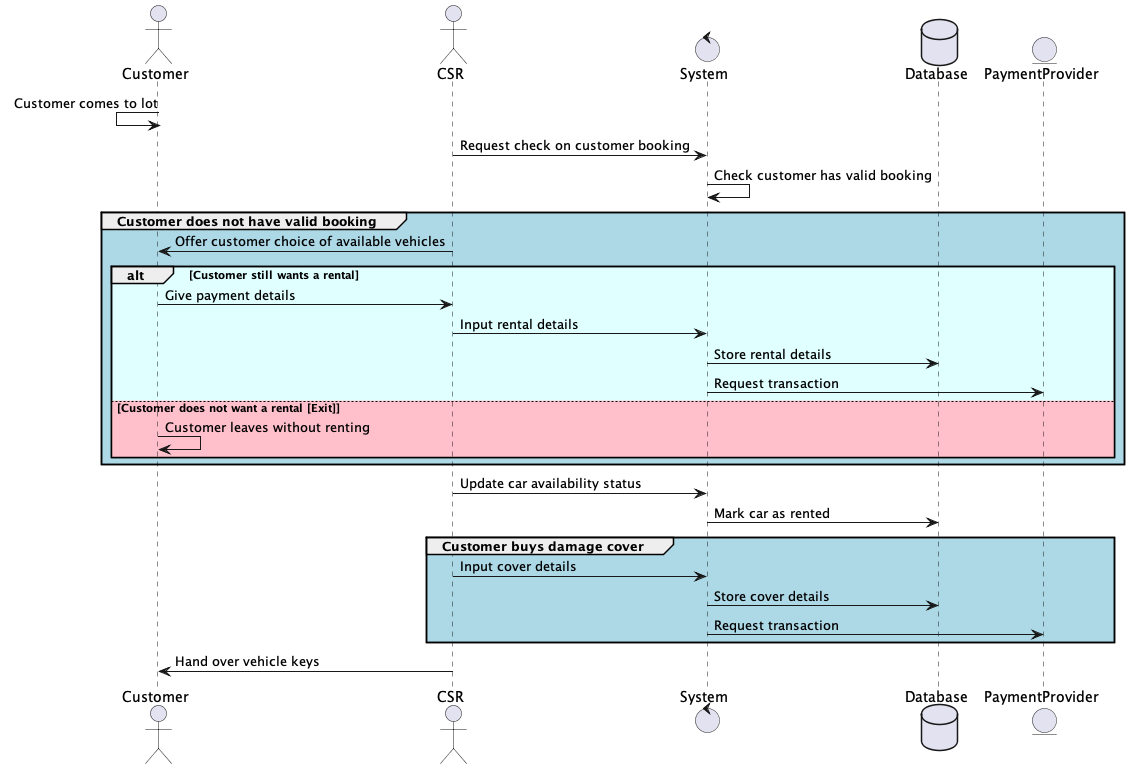
\includegraphics[width=12cm]{assets/Sequence4.png}
    \caption{Sequence diagram for starting a new hire.}
    \label{fig:startHireSequence}
  \end{figure}

  \begin{figure}[H]
    \centering
    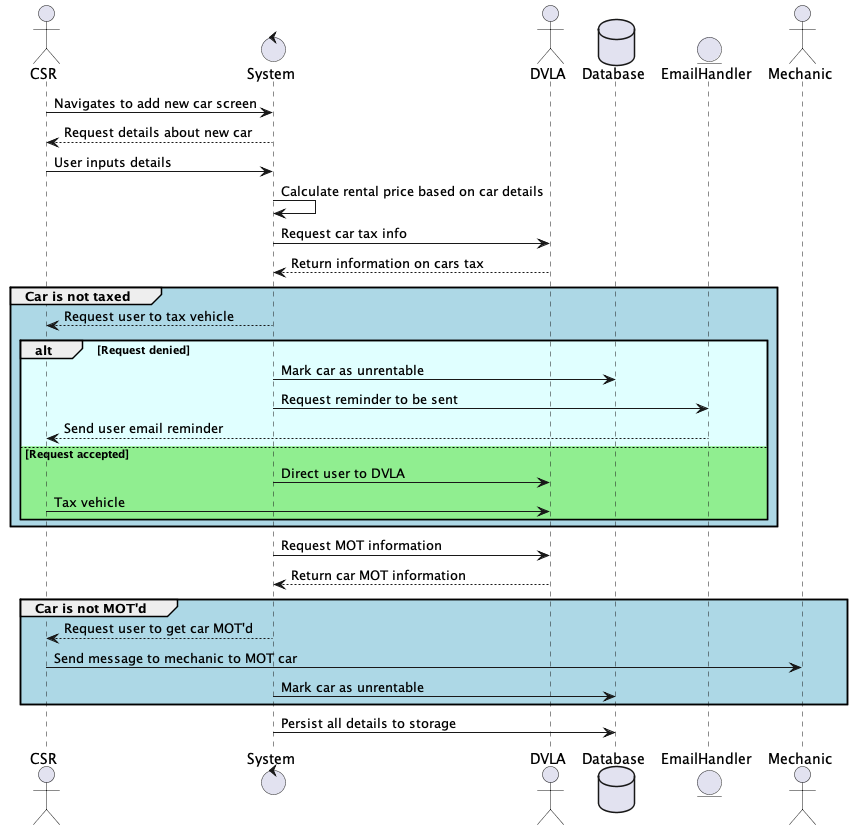
\includegraphics[width=12cm]{assets/Sequence5.png}
    \caption{Sequence diagram for adding a new car to the system.}
    \label{fig:newCarSequence}
  \end{figure}

\subsection{Appendix B - Architectural design of system using AWS}
\label{sec:AppendixB}

  This solution will be built primarily using a cloud-native approach, however as this system is somewhat large there is room for other 
  architectural patterns to be used in sub systems of the overall build. Below is a high level look at how the system could be create using AWS:

  \begin{figure}[H]
    \centering
    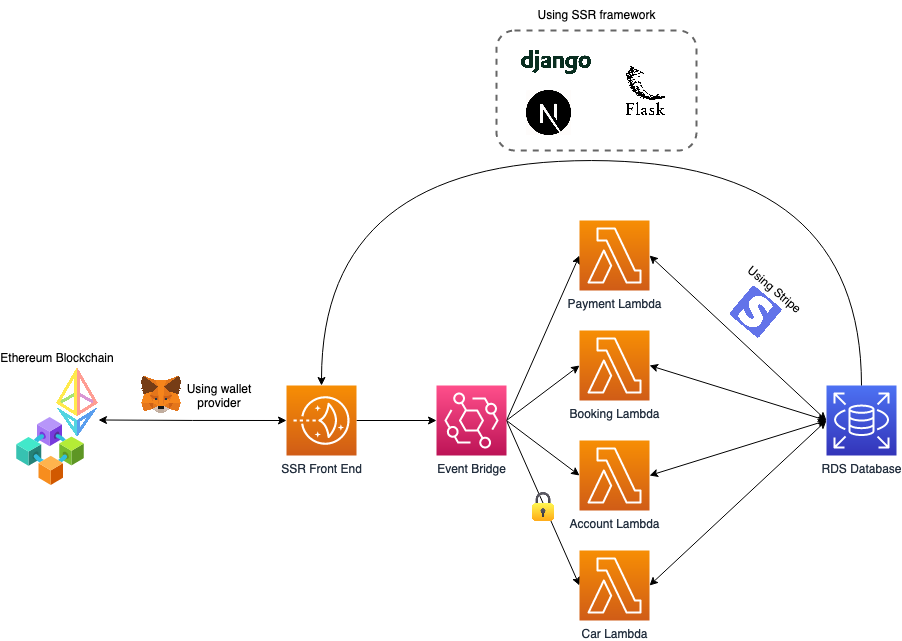
\includegraphics[width=12cm]{assets/architectureEvents.drawio.png}
    \caption{Diagram showing the proposed architecture for the whole system.}
    \label{fig:architecture}
  \end{figure}

  The main component is the Server-side Rendered front end. This can then communicate with the blockchain for crypto transactions using a wallet provider,
  e.g. Metamask [60]. The main functionality is that the front end is then able to send events through EventBridge [61] to individual lambdas [62] for different 
  functionality. These lambdas can then store data into the database. The payment lambda uses Stripe [63] to process payments, and the \textit{'car lambda'} is
  for internal use only, hence the lock on its connection. These topics will be discussed more in the 
  \hyperref[sec:Dependability]{\textbf{Dependability}} section.

\subsection{Appendix C - ACMEs rollback strategy}
\label{sec:AppendixC}

  Rollbacks could be made possible by using Jenkins [64], which is a CI/CD provider. This kind of action should only be taken on components that render the
  service unusable. This automation of rolling back could have other consequences to other systems and therefore should be a last resort and very well 
  tested. For example if a microservice failed, it might not be worth having this automatic process. However if the web front end encountered system failure 
  it'd be worth auto restarting, especially when there is no staff currently working to investigate the problems themselves.
  
  \begin{figure}[H]
    \centering
    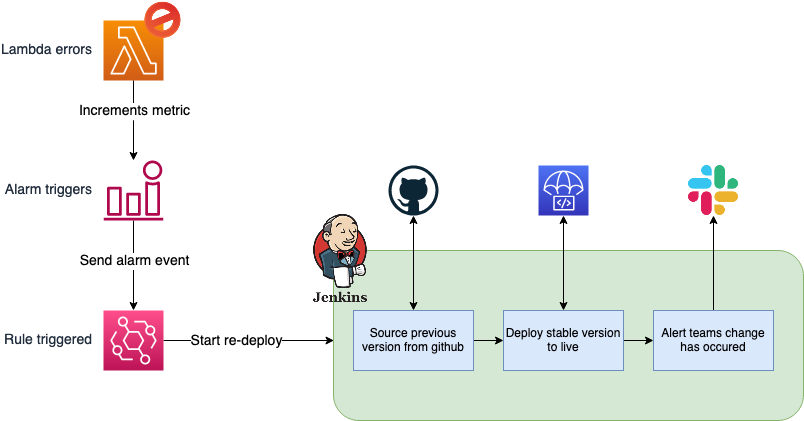
\includegraphics[width=10cm]{assets/rollbackPipeline.drawio.png}
    \caption{Diagram showing how the CI/CD pipeline of a rollback system would operate.}
    \label{fig:rollbackPipeline}
  \end{figure}

\subsection{Appendix D - ACMEs testing strategy}
\label{sec:AppendixD}

  \begin{table}[H]
    \centering
    \begin{tabular}{|l|l|l|}
      \hline
      \textbf{Test Name}    & \textbf{Test Type}  & \textbf{Cadence}  \\ \hline
      UI tests              & E2E                 & Twice a week      \\ \hline
      Booking tests         & Integration         & Daily             \\ \hline
      Payments tests        & Integration         & Daily             \\ \hline     
      Account tests         & Integration         & Daily             \\ \hline     
      Car tests             & Integration         & Daily             \\ \hline   
      P2P/Blockchain tests  & E2E                 & Weekly            \\ \hline 
      Unit tests            & Unit                & On deployment     \\ \hline    
    \end{tabular}
    \caption{Table showing ACMEs tests and testing pattern}
  \end{table}

  The above table shows ACME's testing patterns. Most is quite self-explanatory, the only strange one is that P2P/Blockchain and UI tests are not on 
  the same cadence. This was a decision made due to cost. Blockchains require a gas fee [65] when transacting on them. If this is done on a live 
  environment this is going to cost money to pay that fee. Therefore I have lowered this testing suite down to once a week instead of twice.

\subsection{Appendix E - ACMEs deployment pipeline}
\label{sec:AppendixE}

  \begin{figure}[H]
    \centering
    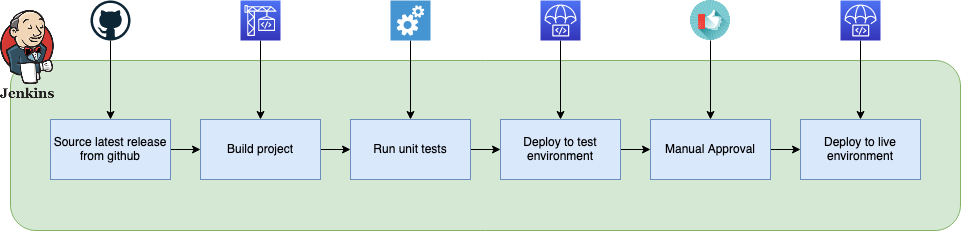
\includegraphics[width=12cm]{assets/relasePipeline.drawio.png}
    \caption{Diagram showing the stages of release for project.}
    \label{fig:releasePipeline}
  \end{figure}

  ACME has its deployment set up in a way where there are two environments, so that new features can be tested in the real world before being pushed to customers.
  First the new code is deployed to test, where it can be double checked and made sure that it is ready by testers. Then, with manual approval, it can be 
  deployed to the live environment. The idea here is having this separation of environments will help catch bugs on the real hardware before going to live.
  There is extra cost to this, however the test environment uses much smaller and cheaper memory and services and is there to check integration between 
  components.
